%!TEX root = ../thesis.tex
\chapter{Appendix}


\begin{figure}[h]
    \centering
    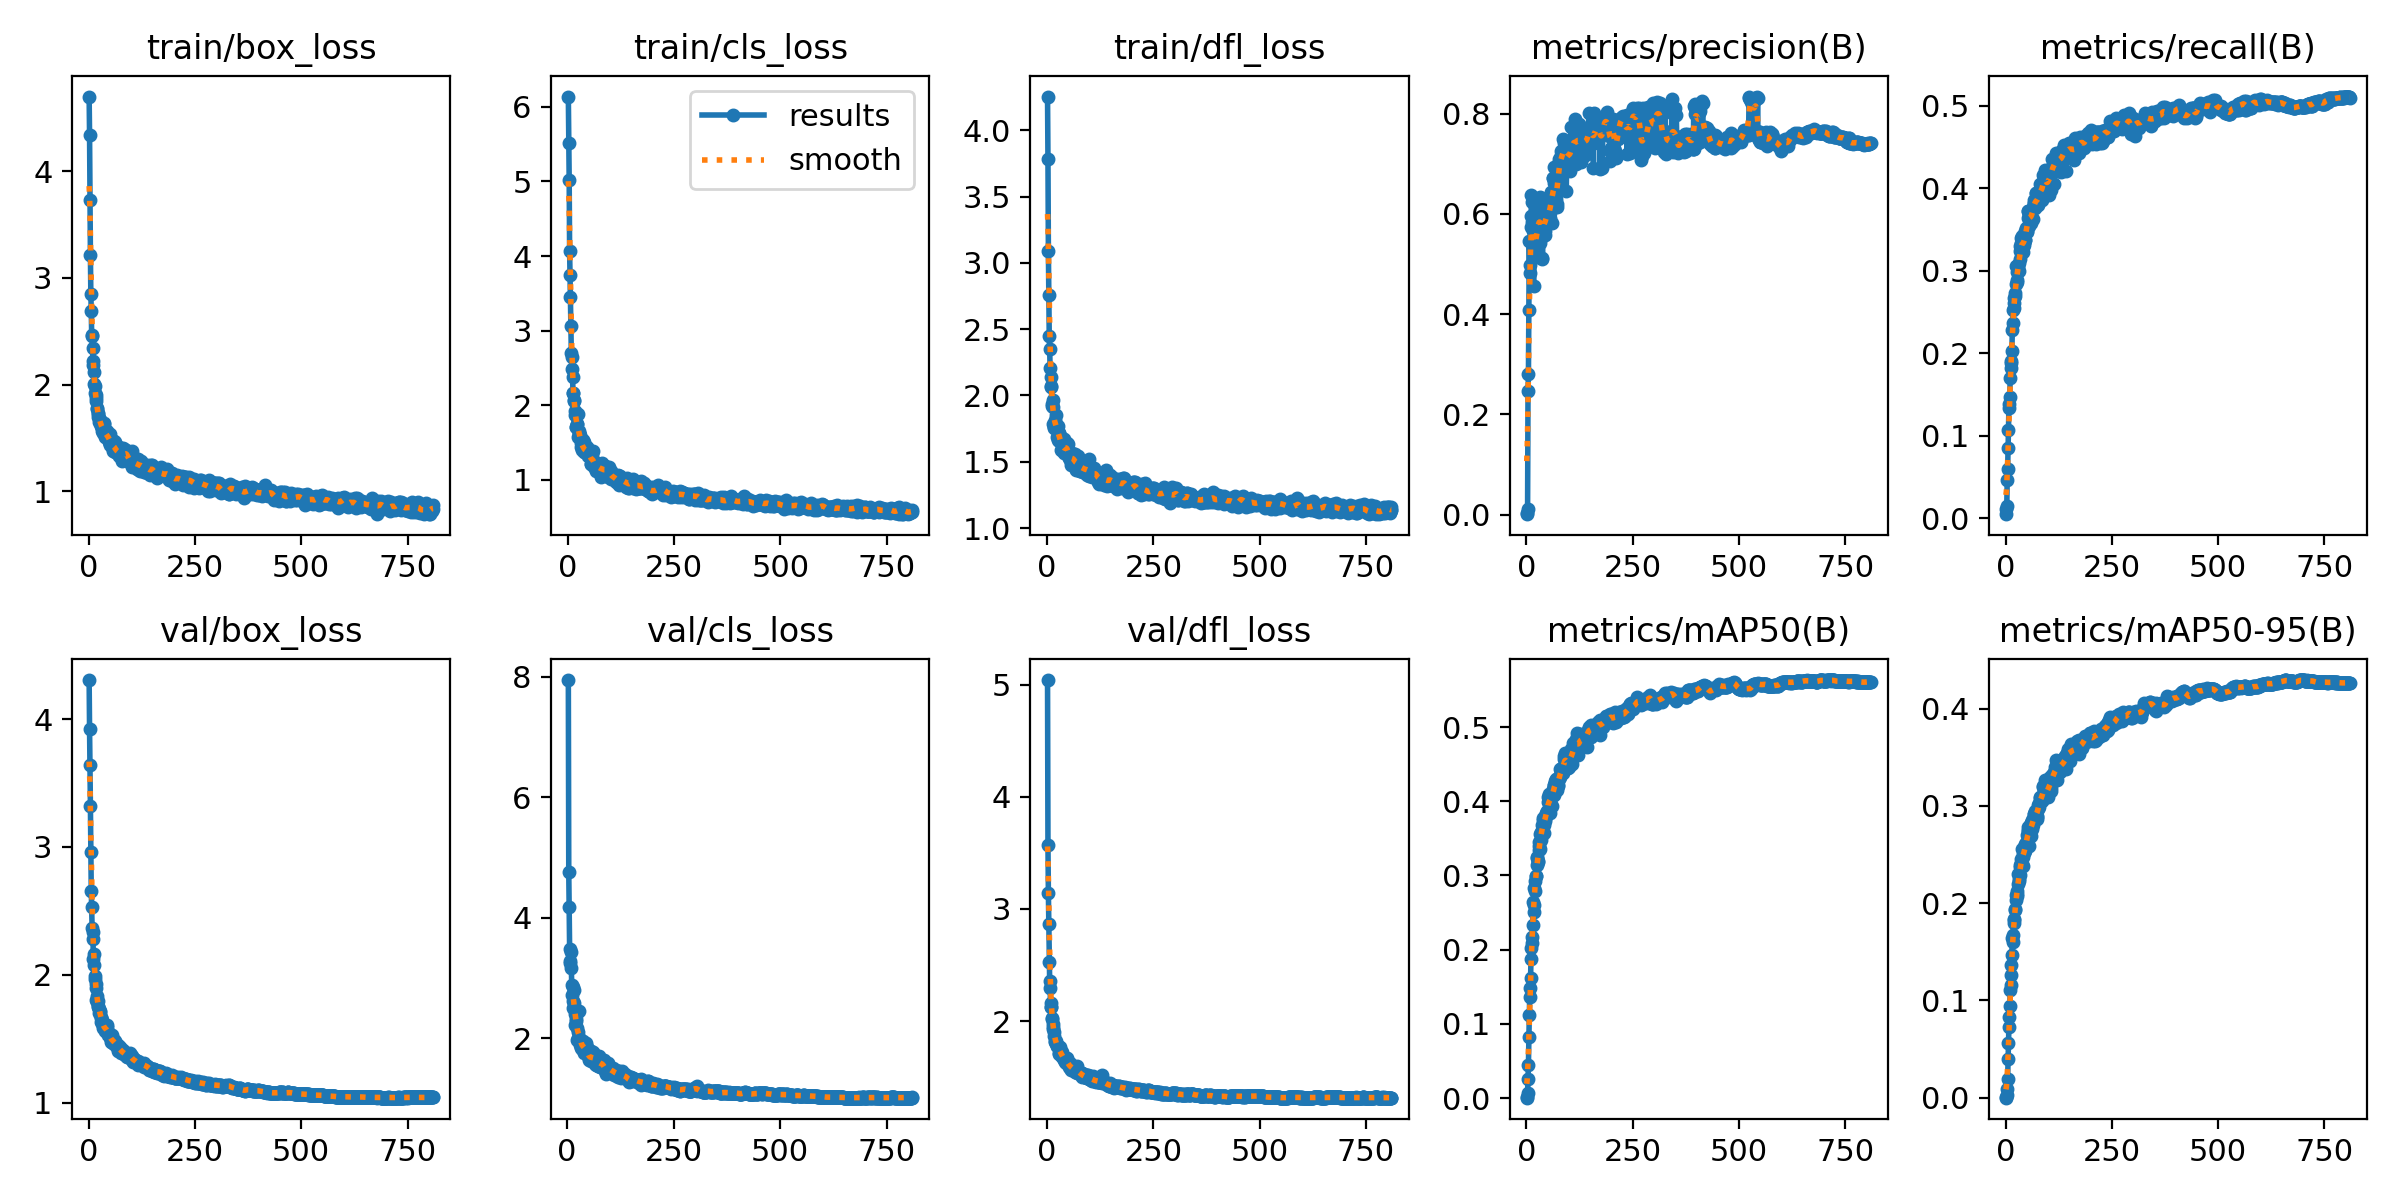
\includegraphics[width=\textwidth]{images/DOTA_train_res.png}
    \caption{Results from \acrshort{DOTA} Training}
    \label{fig:DOTA_train_values}
\end{figure}

\begin{figure}[h]
    \centering
    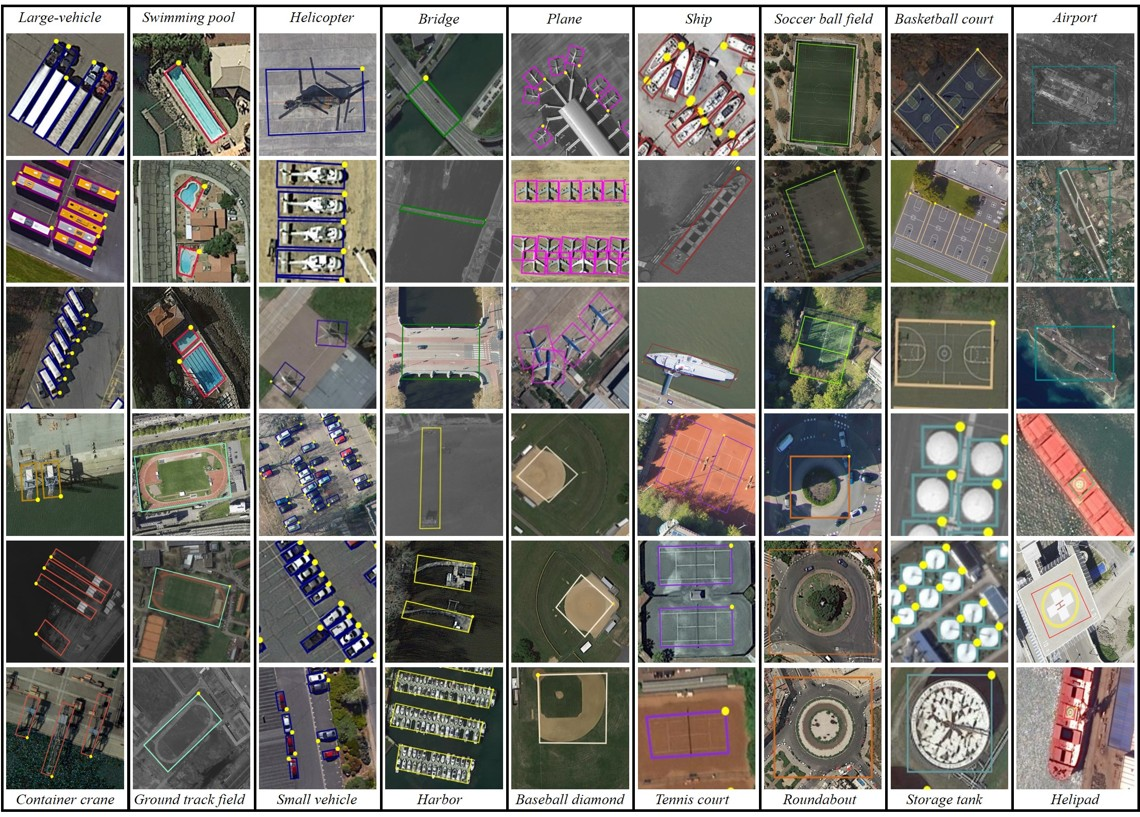
\includegraphics[width=\textwidth]{images/013Methods/class_overview_dota.jpg}
    \caption{Example Classes for DOTA Dataset}
    \label{fig:DOTA_exClasses}
\end{figure}


\section{Full-Sized Images}

\begin{figure}[h]
    \centering
    \begin{subfigure}[b]{0.45\textwidth}
        \centering
        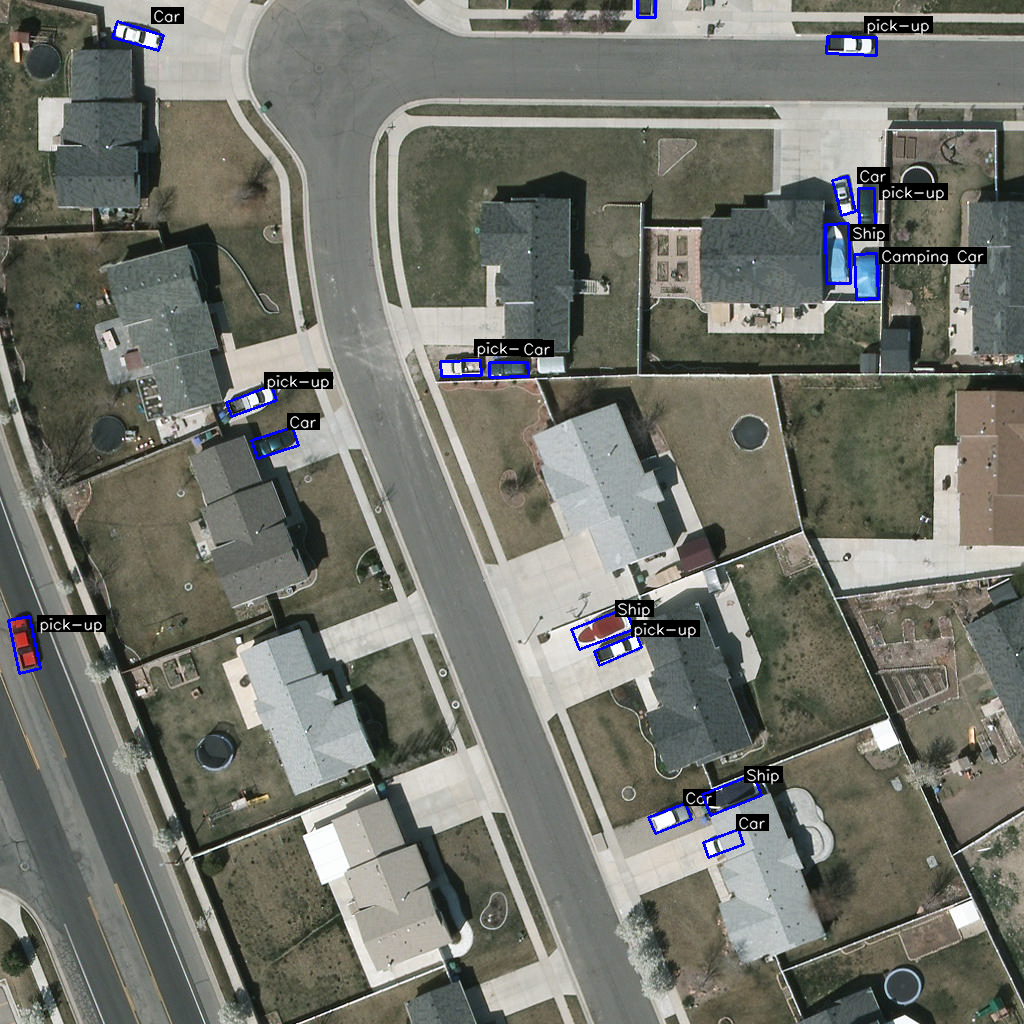
\includegraphics[width=\textwidth]{images/bb_smaller0.png}
        \caption{Two Coordinate out of range and smaller 0}
        \label{fig:smaller0_fs}
    \end{subfigure}
    \hfill
    \begin{subfigure}[b]{0.45\textwidth}
        \centering
        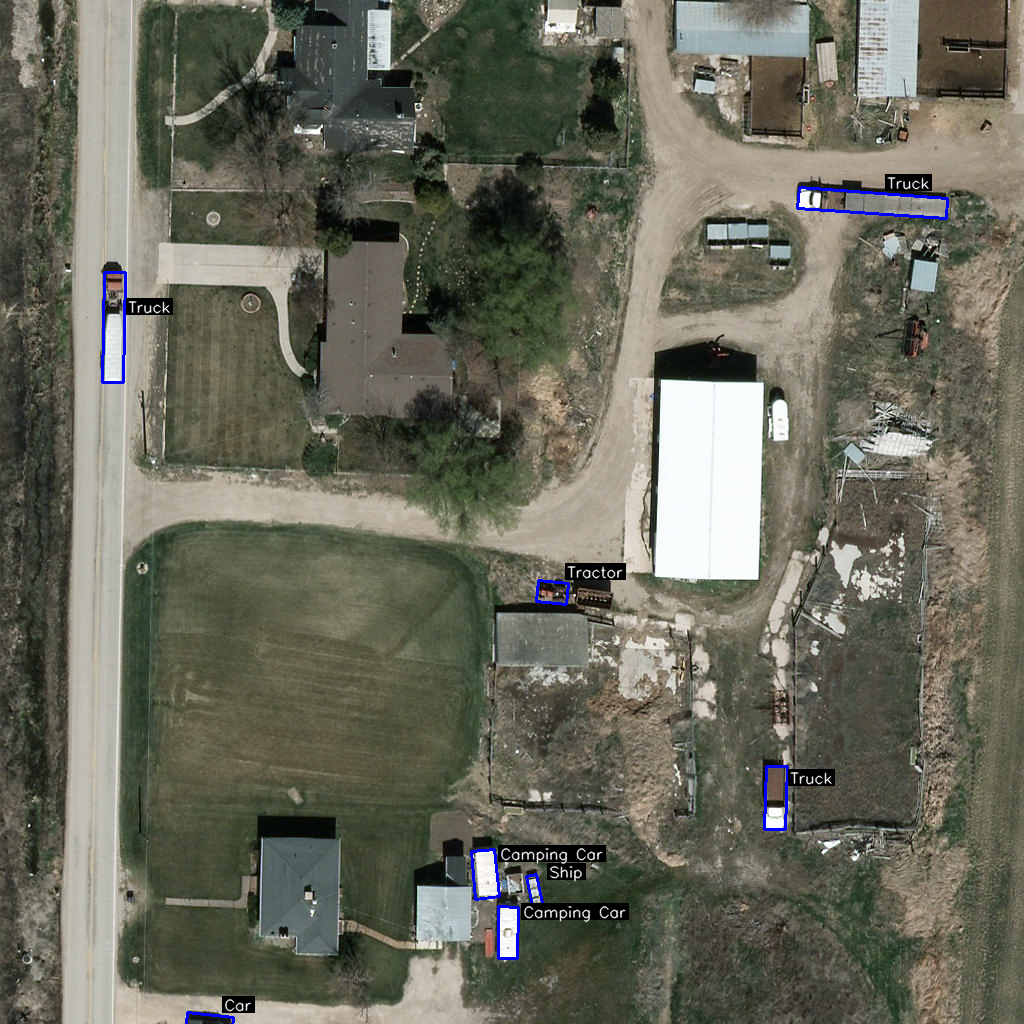
\includegraphics[width=\textwidth]{images/bb_higher1.png}
        \caption{Two Coordinates out ouf range and higher 1}
        \label{fig:higher1_fs}
    \end{subfigure}
    \caption{Example for label coordinates outside of the image (Full-Sized Image)}
    \label{fig:example_coords_ooR_fs}
\end{figure}


\begin{figure}[h]
    \centering
    
    % Erste Zeile
    \begin{subfigure}[b]{0.45\textwidth}
        \centering
        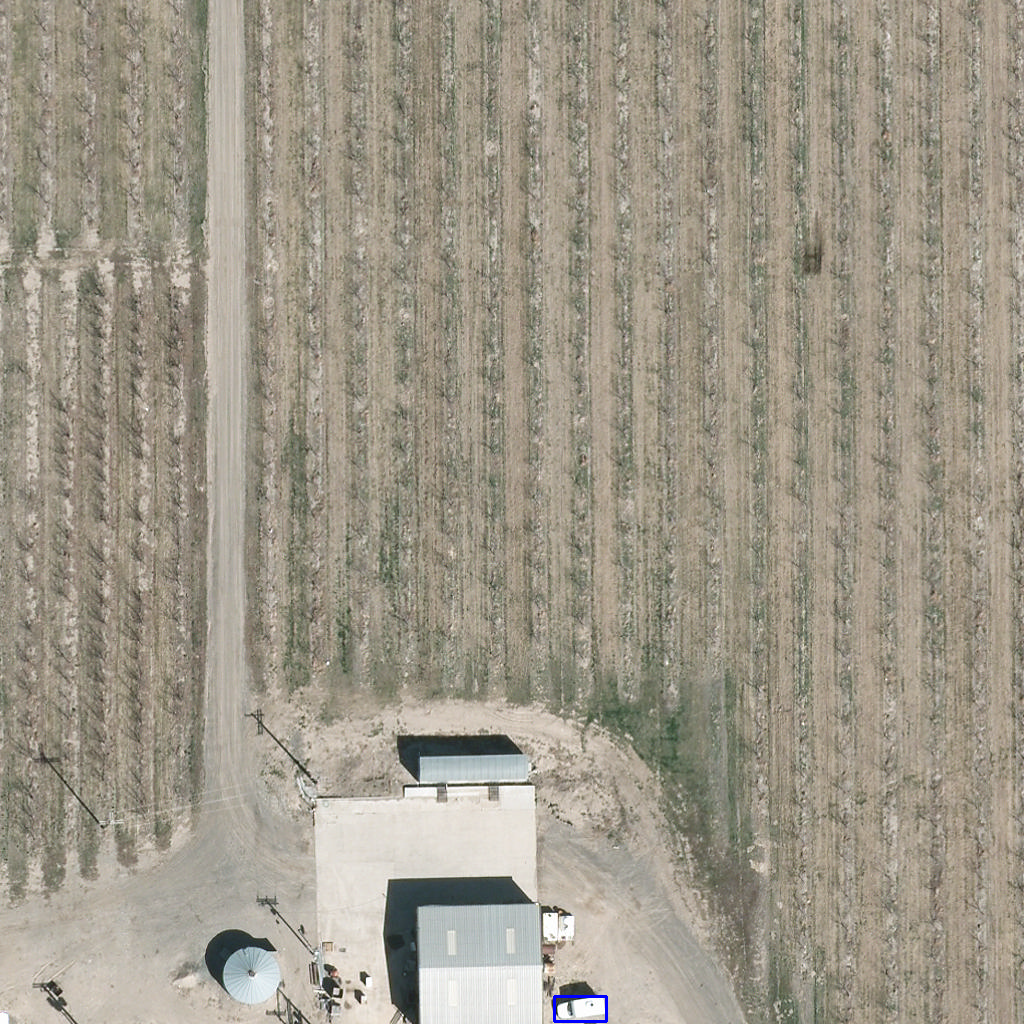
\includegraphics[width=\textwidth]{images/015Results/01abb_vs_obb/abb_truck.png}
        \caption{Label: "Truck", abb format, area: $\approx 1378 \text{px}$}
        \label{fig:abb_truck_fs}
    \end{subfigure}
    \hfill
    \begin{subfigure}[b]{0.45\textwidth}
        \centering
        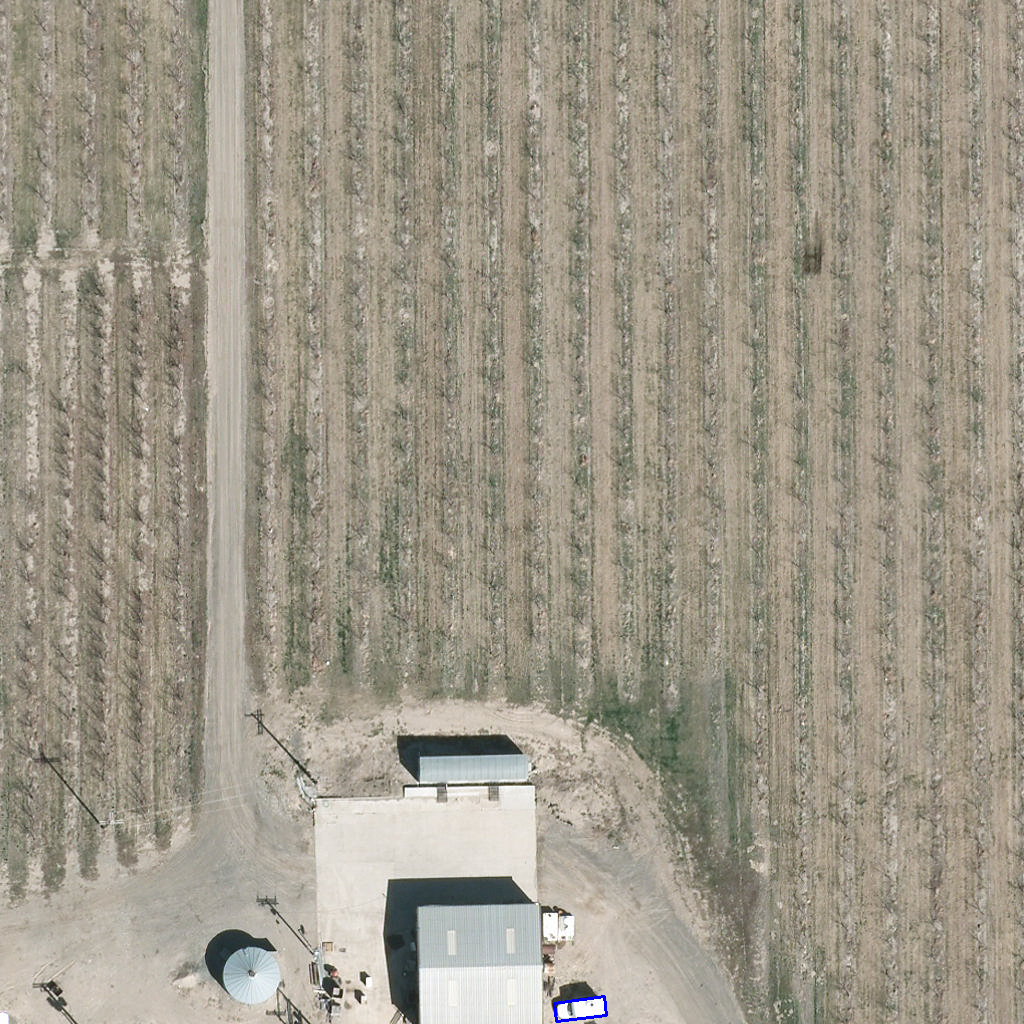
\includegraphics[width=\textwidth]{images/015Results/01abb_vs_obb/obb_truck.png}
        \caption{Label: "Truck", obb format, area: $\approx 967 \text{px}$}
        \label{fig:obb_truck_fs}
    \end{subfigure}
    
    \vspace{0.5cm} % Abstand zwischen den Zeilen
    
    % Zweite Zeile
    \begin{subfigure}[b]{0.45\textwidth}
        \centering
        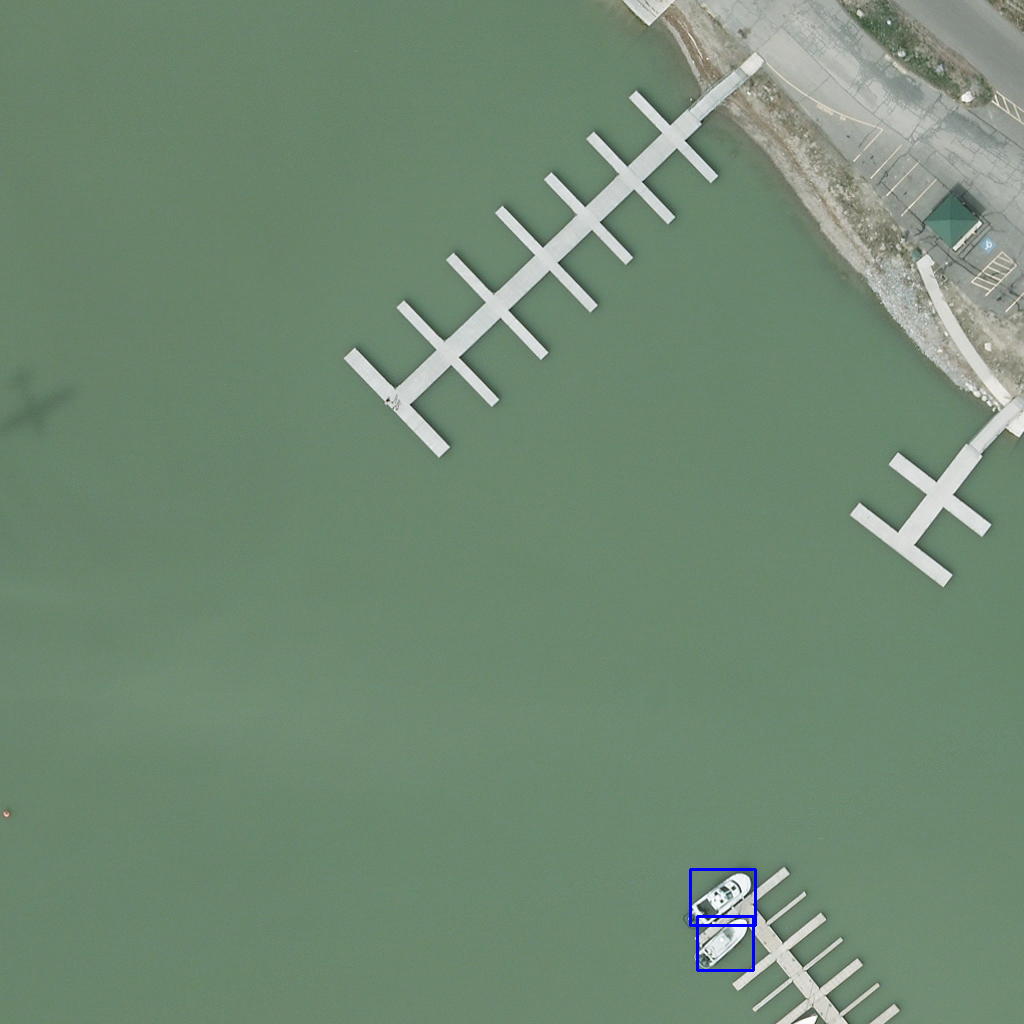
\includegraphics[width=\textwidth]{images/015Results/01abb_vs_obb/abb_ship.png}
        \caption{Labels: "Ship", abb format}
        \label{fig:abb_ship_fs}
    \end{subfigure}
    \hfill
    \begin{subfigure}[b]{0.45\textwidth}
        \centering
        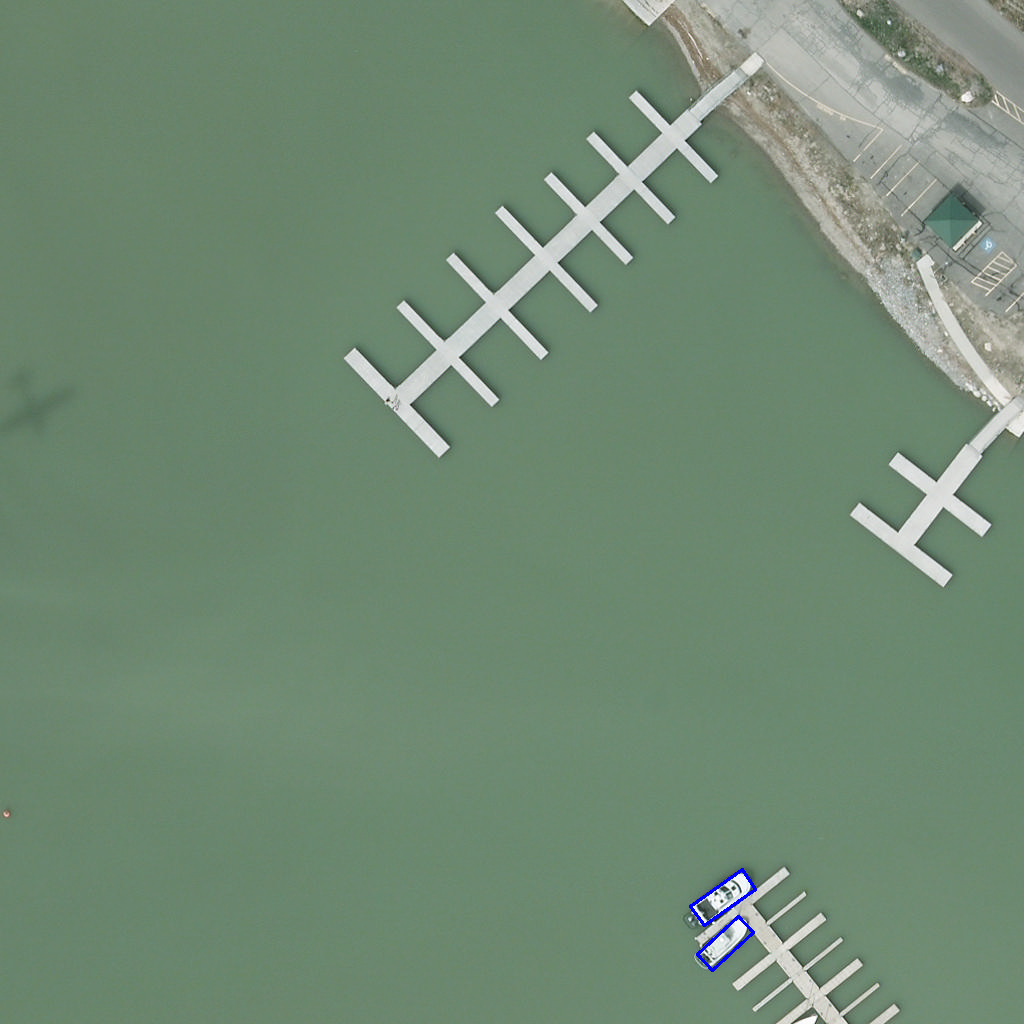
\includegraphics[width=\textwidth]{images/015Results/01abb_vs_obb/obb_ship.png}
        \caption{Labels: "Ship", obb format}
        \label{fig:obb_ship_fs}
    \end{subfigure}  
    \caption{Comparison of the bounding box formats of two different object classes (Full-Sized)}
    \label{fig:comparison_bb_format_fs}
\end{figure}

\clearpage

\section{Results}
\subsection{Calculation Bounding Box Area in Percent}
\label{ap:calc_bb_area_percent}

The total area of the image ($A_{\text{total}}$) is $1024 \times 1024 = 1,048,576 \text{ pixels}^2$.

\subsubsection*{Calculation of Bounding Box Area in Percent}
The percentage area ($F_{\%}$) is calculated using the following formula:
$$F_{\%} = \frac{A_{\text{Box}}}{A_{\text{total}}} \times 100\%$$

\subsubsection*{OBB (Oriented Bounding Box)}
The median area is $\approx 700$ pixels.
$$F_{\%,\text{obb}} = \frac{700}{1,048,576} \times 100\% \approx 0.06675\%$$

\subsubsection*{ABB (Axis-aligned Bounding Box)}
The median area is $\approx 1000$ pixels.
$$F_{\%,\text{abb}} = \frac{1000}{1,048,576} \times 100\% \approx 0.09536\%$$



\subsection{Additional Tables}

\begin{table}[h!]
\centering
\begin{tabular}{cc}
\hline
\textbf{Class} & \textbf{Color} \\
\hline
\acrfull{GT} & \tikz\fill[GroundTruthColor] (0,0) rectangle (0.5cm,0.3cm); \\
Car        & \tikz\fill[CarColor] (0,0) rectangle (0.5cm,0.3cm); \\
Truck      & \tikz\fill[TruckColor] (0,0) rectangle (0.5cm,0.3cm); \\
Ship       & \tikz\fill[ShipColor] (0,0) rectangle (0.5cm,0.3cm); \\
Tractor    & \tikz\fill[TractorColor] (0,0) rectangle (0.5cm,0.3cm); \\
Camping Car & \tikz\fill[CampingCarColor] (0,0) rectangle (0.5cm,0.3cm); \\
Van        & \tikz\fill[VanColor] (0,0) rectangle (0.5cm,0.3cm); \\
Vehicle    & \tikz\fill[VehicleColor] (0,0) rectangle (0.5cm,0.3cm); \\
Pick-up    & \tikz\fill[PickUpColor] (0,0) rectangle (0.5cm,0.3cm); \\
Plane      & \tikz\fill[PlaneColor] (0,0) rectangle (0.5cm,0.3cm); \\
\hline
\end{tabular}
\caption{Classes with corresponding colors, including \acrshort{GT}}
\label{tab:class_colors}
\end{table}

\begin{table}[h!]
\centering
\begin{tabular}{c|c}
\hline
\textbf{Vehicle Type} & \textbf{freq\_val} \\
\hline
Car & 0 \\
Pick Up & 1 \\
Camping Car & 2 \\
Truck & 3 \\
Vehicle & 4 \\
Tractor & 5 \\
Ship & 6 \\
Van & 7 \\
Plane & 8 \\
\hline
\end{tabular}
\caption{Vehicle types and their corresponding freq\_val (Frequency Value) assignments}
\label{tab:class_freq_val}
\end{table}




\begin{table}[h!]
\centering

\begin{tabular}{c|c|c|c|c|c|c}
\hline
Val-Fold & Train-Folds & \#Train-Objects & Plane (Train) & Plane (Val) & CV$_{train}$ & max/min$_{train}$ \\
\hline
0 & 1,2,3,4 & 2531 & 37 & 4  & 1.0124 & 25.14 \\
1 & 0,2,3,4 & 2502 & 30 & 11 & 1.0200 & 30.67 \\
2 & 0,1,3,4 & 2542 & 37 & 4  & 1.0142 & 25.22 \\
3 & 0,1,2,4 & 2524 & 23 & 18 & 1.0253 & 40.61 \\
4 & 0,1,2,3 & 2525 & 37 & 4  & 1.0073 & 24.84 \\
\hline
\end{tabular}
\caption[Classbalance at 6-Fold Cross Validation]{Classbalance at 6-Fold Cross Validation (Fold 5 is Testdataset)}
\end{table}


% \begin{landscape}
% \begin{table}[ht!]
%     \centering
%     \adjustbox{max width=\linewidth}{%
%     \begin{tabular}{c|ccc|ccc|ccc|ccc|ccc}
%     \hline
%     & \multicolumn{3}{c|}{Val=0} & \multicolumn{3}{c|}{Val=1} & \multicolumn{3}{c|}{Val=2} & \multicolumn{3}{c|}{Val=3} & \multicolumn{3}{c}{Val=4} \\
%     Klasse & Train & Val & Test & Train & Val & Test & Train & Val & Test & Train & Val & Test & Train & Val & Test \\
%     \hline
%     Car        & 934 & 229 & 225 & 930 & 239 & 225 & 933 & 226 & 225 & 934 & 225 & 225 & 934 & 240 & 225 \\
%     Truck      & 207 & 51  & 50  & 201 & 57  & 50  & 208 & 50  & 50  & 208 & 49  & 50  & 207 & 51  & 50 \\
%     Ship       & 117 & 30  & 27  & 116 & 28  & 27  & 115 & 29  & 27  & 114 & 30  & 27  & 117 & 27  & 27 \\
%     Tractor    & 123 & 30  & 30  & 124 & 32  & 30  & 126 & 33  & 30  & 124 & 30  & 30  & 125 & 31  & 30 \\
%     Campingcar & 269 & 65  & 63  & 262 & 72  & 63  & 270 & 64  & 63  & 267 & 69  & 63  & 265 & 64  & 63 \\
%     Van        & 67  & 18 & 16 & 68  & 17 & 16 & 68  & 17 & 16 & 68  & 17 & 16 & 69  & 16 & 16 \\
%     Vehicle    & 144 & 34 & 33 & 141 & 37 & 33 & 144 & 34 & 33 & 144 & 34 & 33 & 145 & 39 & 33 \\
%     Pick-Up    & 637 & 164 & 157 & 640 & 161 & 157 & 644 & 157 & 157 & 641 & 160 & 157 & 642 & 159 & 157 \\
%     Plane      & 37  & 4  & 7  & 30  & 11 & 7  & 37  & 4  & 7  & 23  & 18 & 7  & 37  & 4  & 7 \\
%     \hline
%     \end{tabular}%
%     }
%     \caption[Class distribution (train/val/test) for 6-fold CV]{Class distribution (train/val/test) for 6-fold CV with fold 5 as test -- All classes}
% \end{table}